%!TEX root = ./ERL Industrial Robots.tex


%--------------------------------------------------------------------
%--------------------------------------------------------------------
\subsection{Objects in the Environment}
\label{ssec:Objects}

The objects to be manipulated will be selected by the organizer for each tournament.
The following lists describe the different categories of objects that can be used by
the organizer to use during a tournament depending upon the scenario being choosen.
The different categories of objects are:
%
\begin{itemize}
\item Robocup objects 
\item T-LESS dataset objects
\item Chocolate objects
\end{itemize} 
%
%These objects are listed in Table \ref{tab:DriveAxlePartsRulebook} and \ref{tab:ObjectsToRecognize}.

%--------------------------------------------------------------------
\subsubsection{Manipulation Objects}
\label{sssec:PartstoManipulate}
\newcommand*{\ObjectTablePartsImageScale}{0.12\textwidth}

\begin{figure}[hht]
\centering
\subfigure[Bearing Box]{

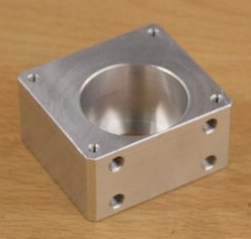
\includegraphics[width=\ObjectTablePartsImageScale, trim=0px 0px 0px -20px, clip] {pics/atwork/objects/bearingBoxA.jpg}
   \label{fig:subfig1}
}
\subfigure[Motor]{
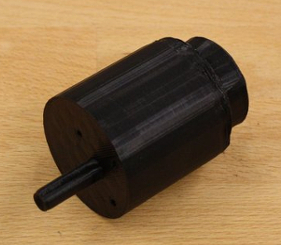
\includegraphics[width=\ObjectTablePartsImageScale, trim=0px 0px 0px -20px, clip] {pics/atwork/objects/motor.jpg} 
   \label{fig:subfig2}
}
\subfigure[Axis]{
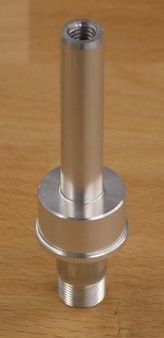
\includegraphics[width=\ObjectTablePartsImageScale, trim=0px 0px 0px -20px, clip] {pics/atwork/objects/axis.jpg} 	
   \label{fig:subfig3}
}
\subfigure[Bearing]{
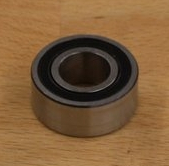
\includegraphics[width=\ObjectTablePartsImageScale, trim=0px 0px 0px -20px, clip] {pics/atwork/objects/bearing.jpg}%		& \texttt{Bearing} 	    		\\  \hline   
   \label{fig:subfig4}
}

\subfigure[F20\_20\_B]{
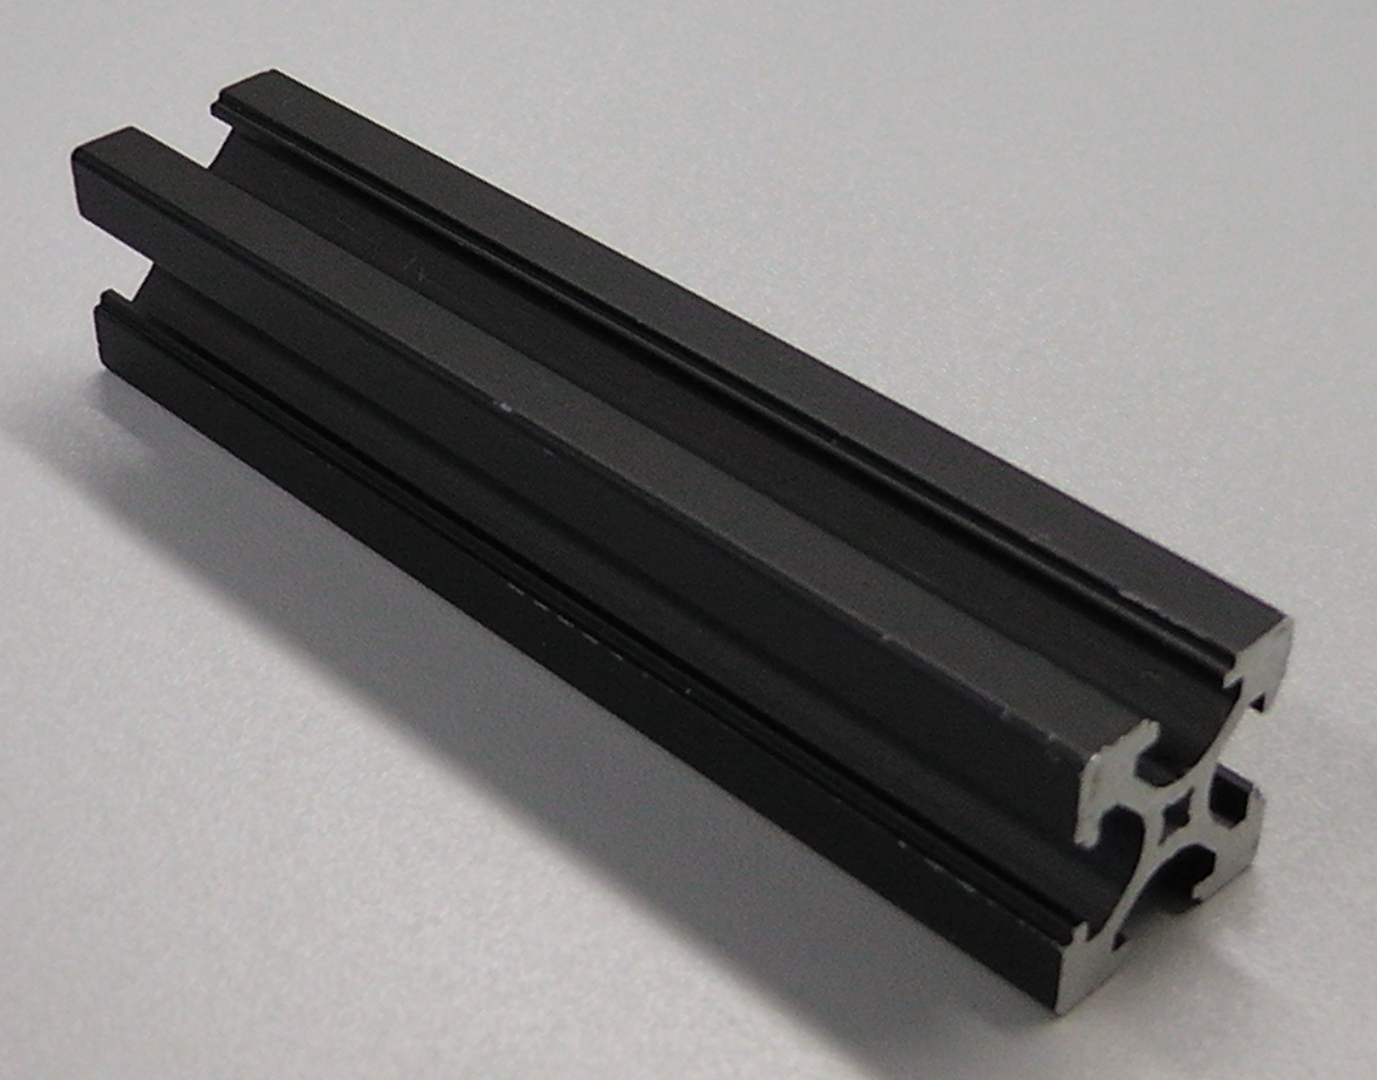
\includegraphics[width=\ObjectTablePartsImageScale, trim=0px 0px 0px -20px, clip] {pics/atwork/objects/F20_20_B.jpg} %	& \texttt{F20\_20\_B}			\\  \hline 
   \label{fig:subfig6}
}
\subfigure[F20\_20\_G]{
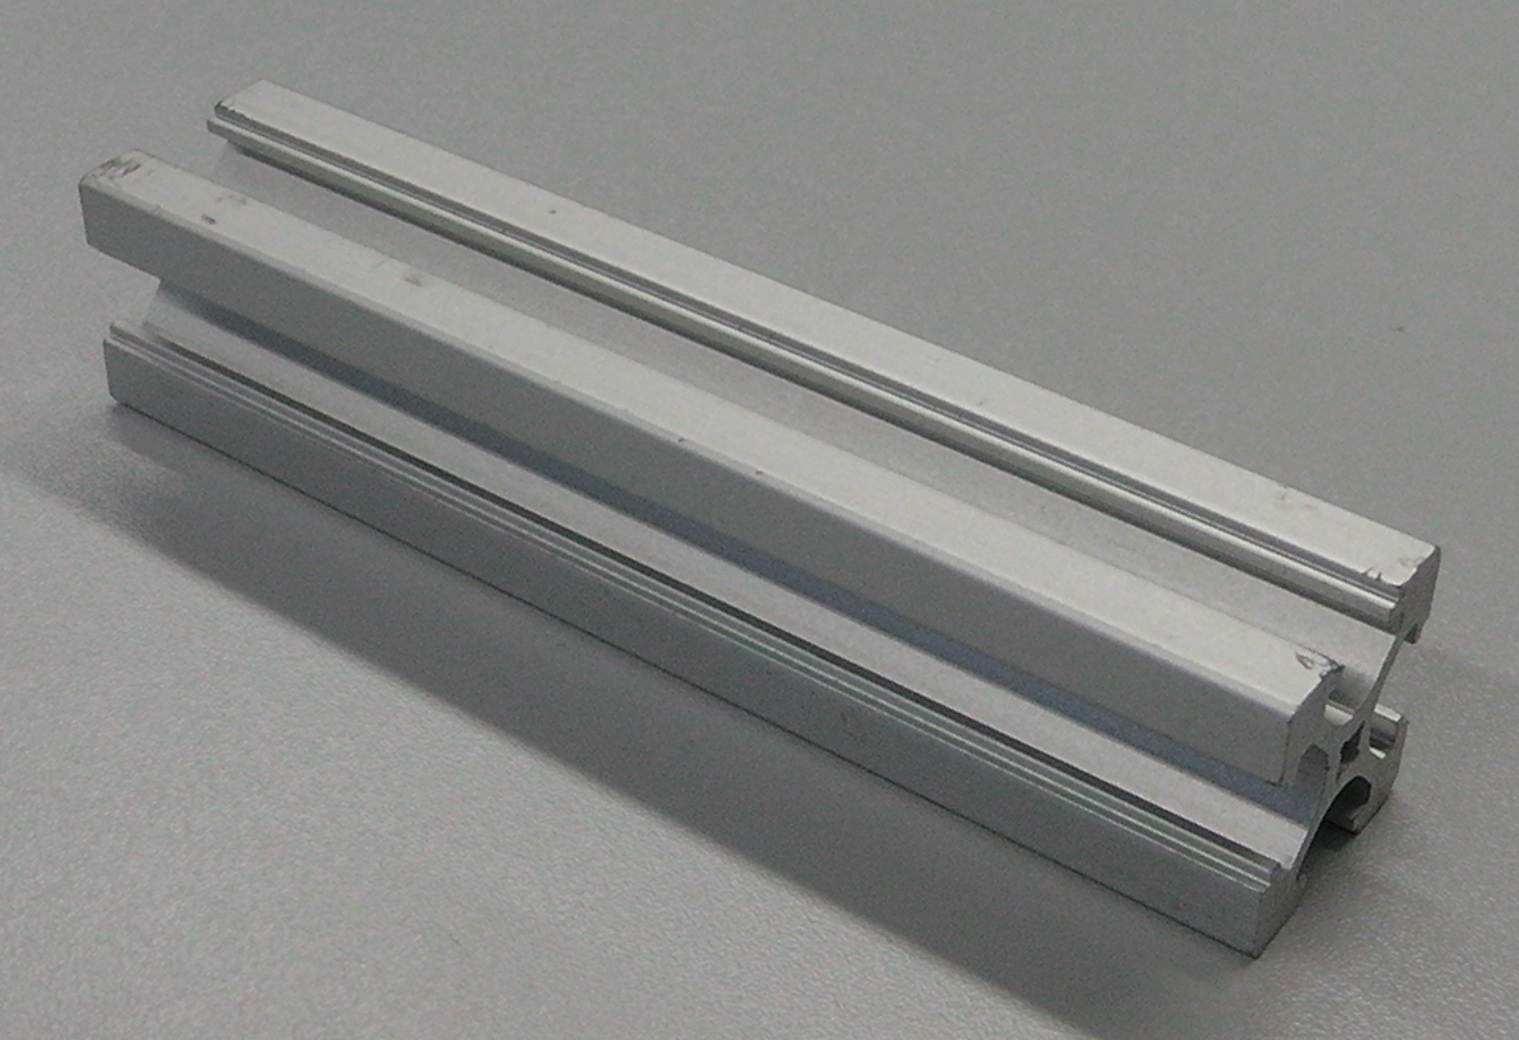
\includegraphics[width=\ObjectTablePartsImageScale, trim=0px 0px 0px -20px, clip] {pics/atwork/objects/F20_20_G.jpg} %	& \texttt{F20\_20\_G}			\\  \hline 
   \label{fig:subfig7}
}
\subfigure[S40\_40\_B]{
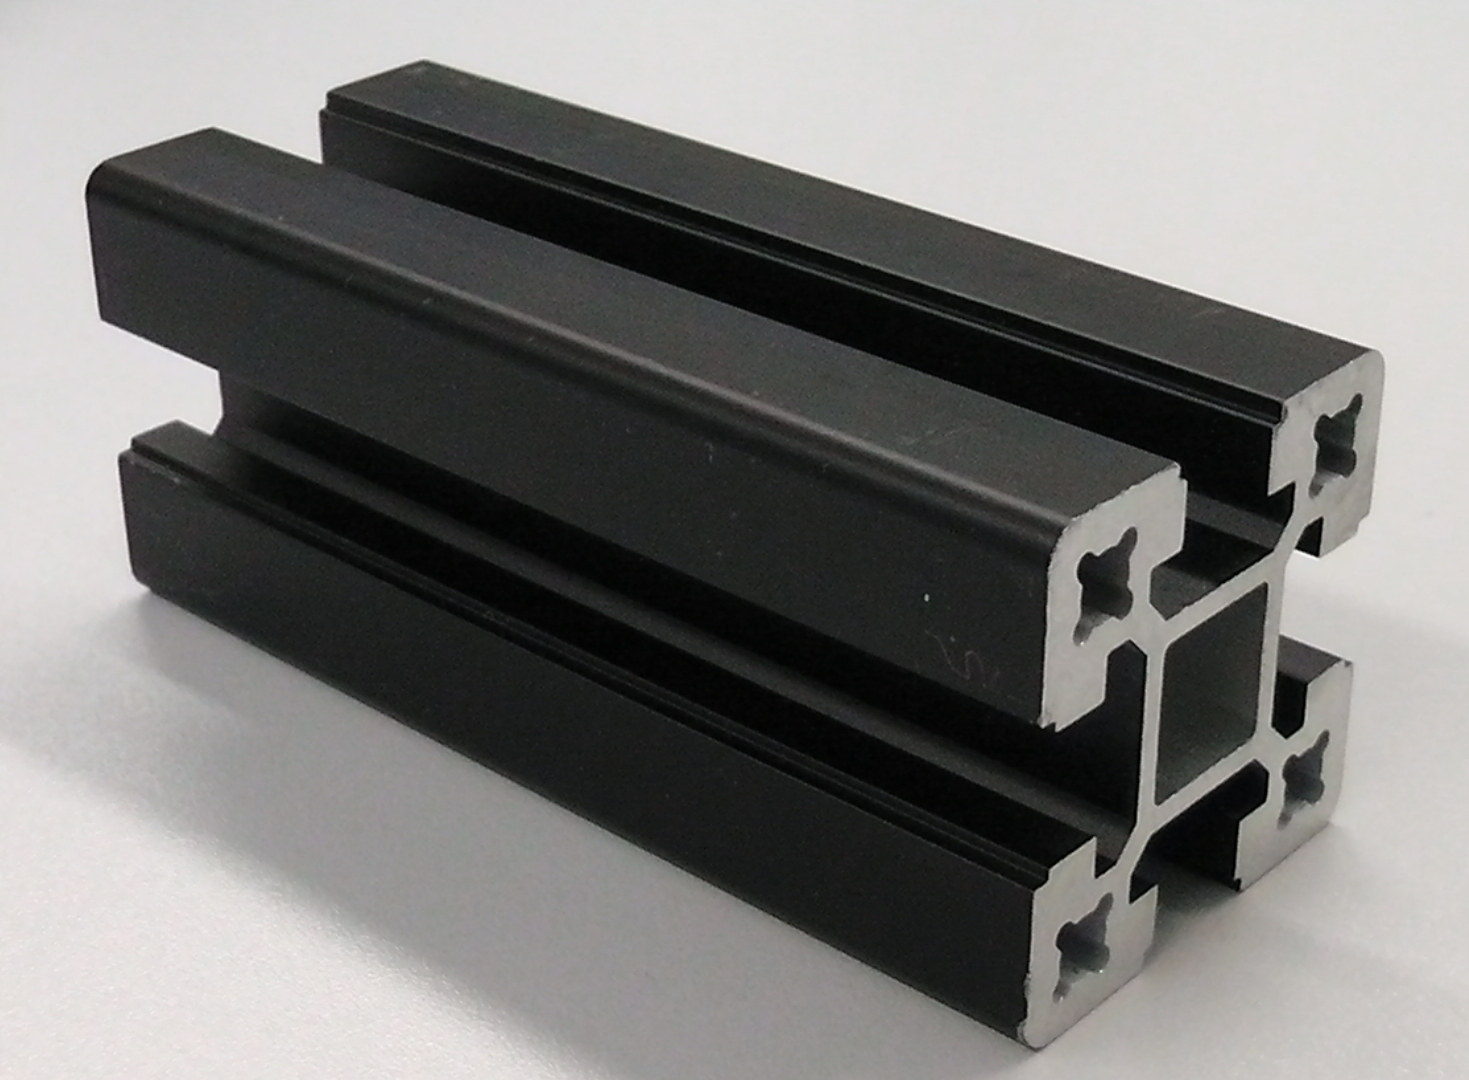
\includegraphics[width=\ObjectTablePartsImageScale, trim=0px 0px 0px -20px, clip] {pics/atwork/objects/S40_40_B.jpg} %	& \texttt{S40\_40\_B}			\\  \hline 
   \label{fig:subfig8}
}
\subfigure[S40\_40\_G]{
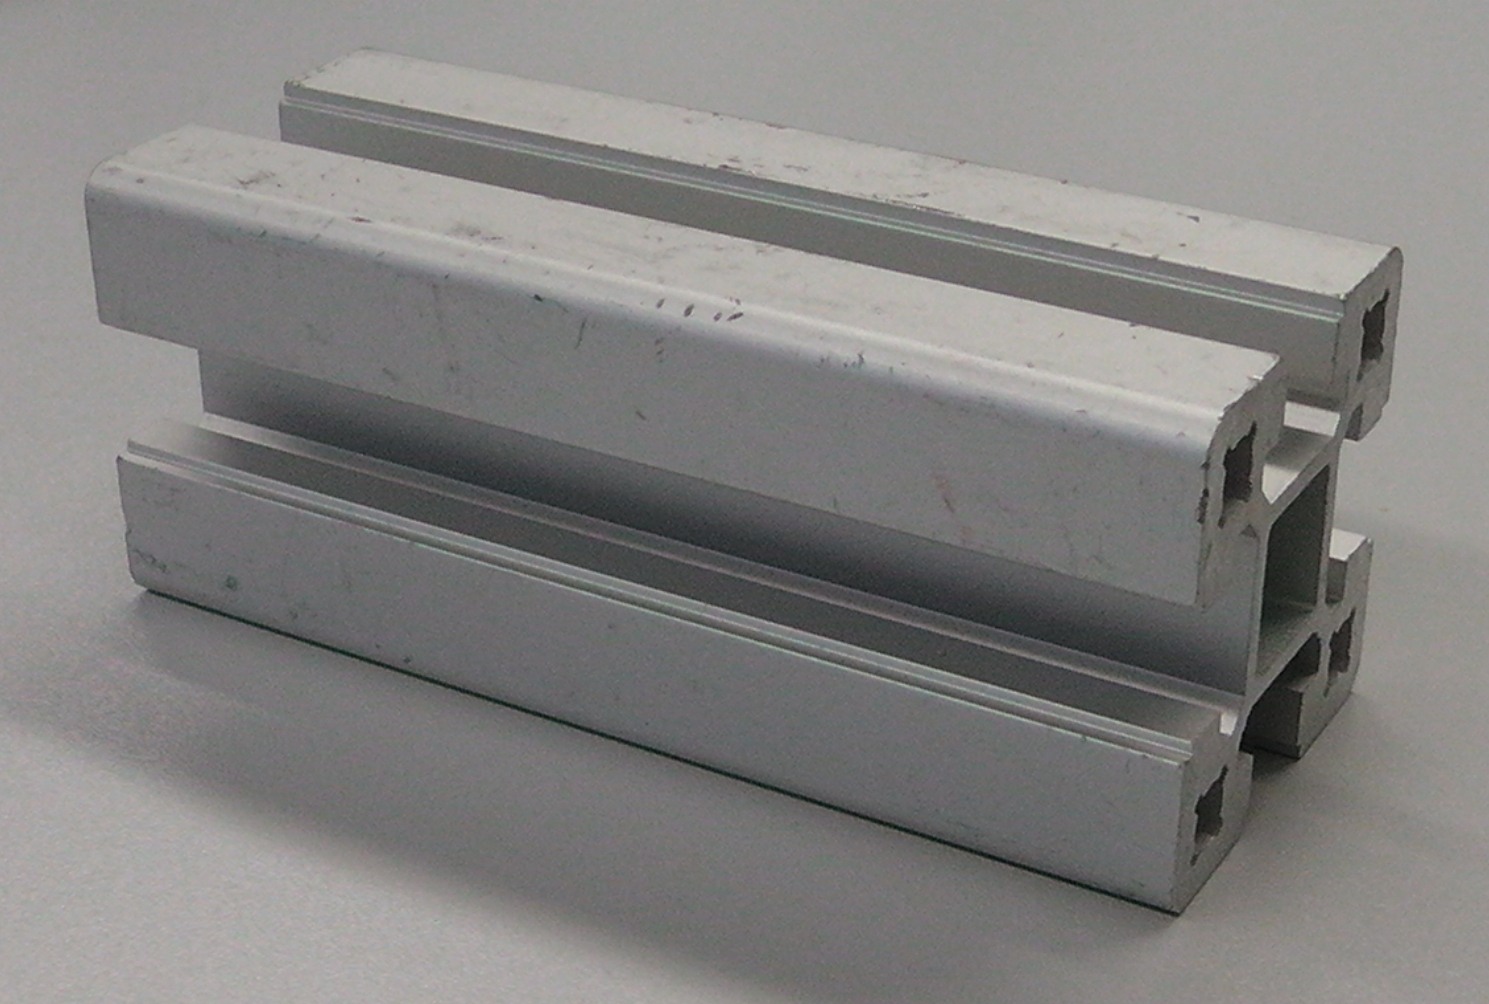
\includegraphics[width=\ObjectTablePartsImageScale, trim=0px 0px 0px -20px, clip] {pics/atwork/objects/S40_40_G.jpg} %	& \texttt{S40\_40\_G}			\\  \hline 
   \label{fig:subfig9}
}
\subfigure[M20\_100]{
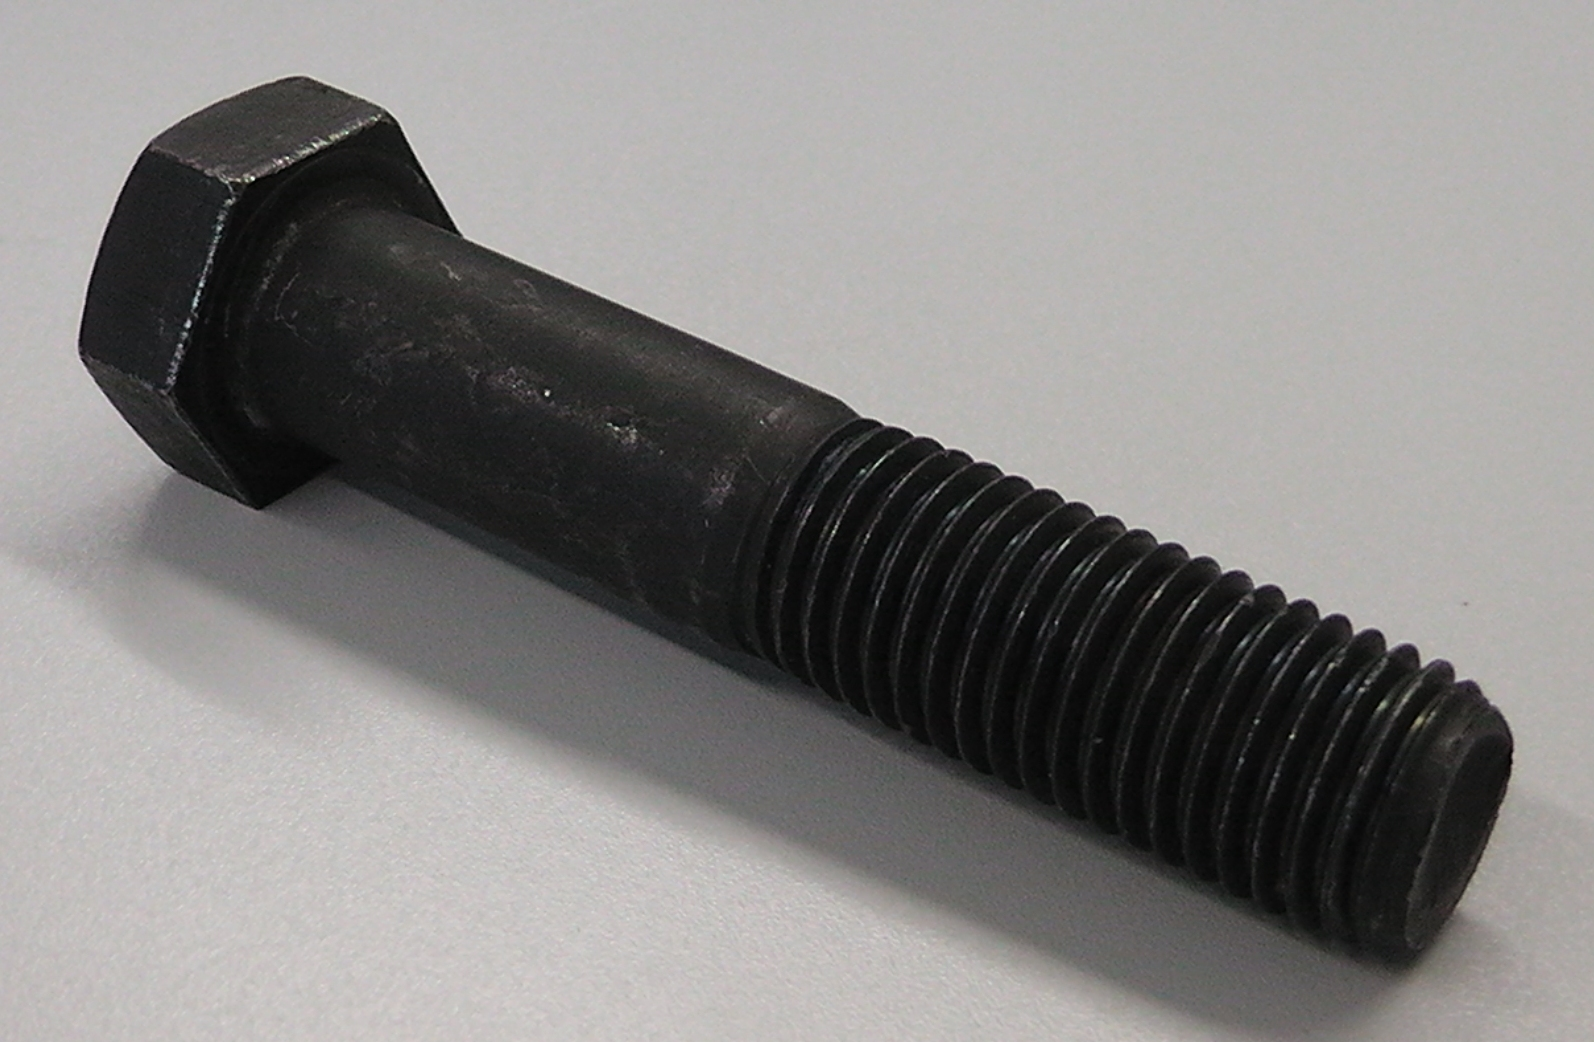
\includegraphics[width=\ObjectTablePartsImageScale, trim=0px 0px 0px -20px, clip] {pics/atwork/objects/M20_100.jpg} 	%	& \texttt{M20\_100}				\\  \hline 
   \label{fig:subfig10}
}
\subfigure[M20]{
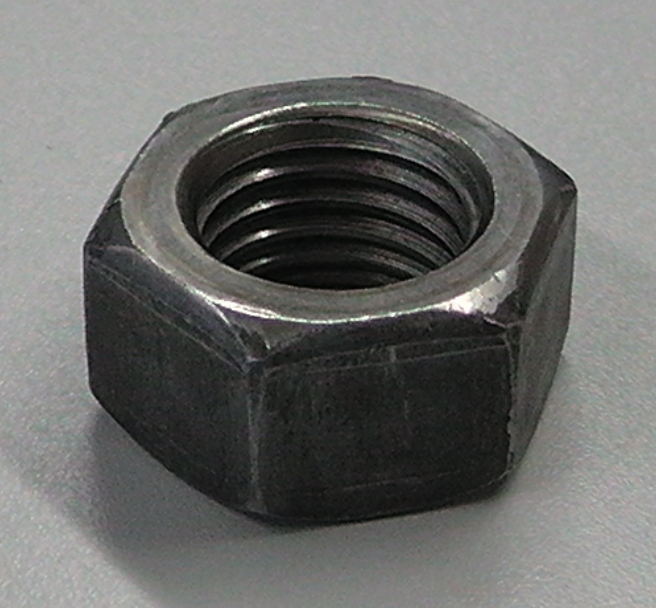
\includegraphics[width=\ObjectTablePartsImageScale, trim=0px 0px 0px -20px, clip] {pics/atwork/objects/M20.jpg} 	%		& \texttt{M20}					\\  \hline 
   \label{fig:subfig11}
}
\subfigure[Distance\_Tube]{
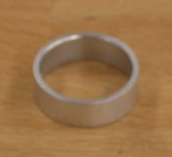
\includegraphics[width=\ObjectTablePartsImageScale, trim=0px 0px 0px -20px, clip] {pics/atwork/objects/distanceTube.jpg}% & \texttt{Distance\_Tube}		\\  \hline   
   \label{fig:subfig5}
}
\caption[Robocup Objects]{Robocup Objects }
\label{fig:labelHere}
\end{figure}

%--------------------------------------------------------------------

\begin{figure}[hh!t]
\centering
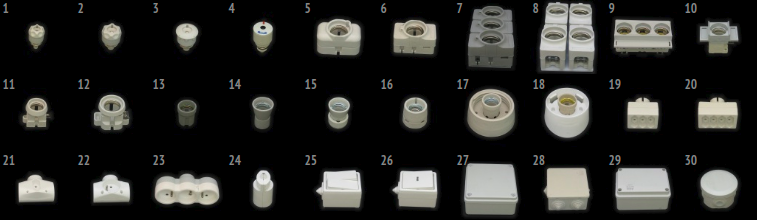
\includegraphics[width=0.8\textwidth, trim=0px 0px 0px -20px, clip] {pics/atwork/objects/t-less.png} 
\caption[T-less dataset objects (http://cmp.felk.cvut.cz/t-less/)]{T-less dataset }
\label{fig:labelHere}
\end{figure}

%--------------------------------------------------------------------


\begin{figure}[hh!t]
\centering
\subfigure[]{
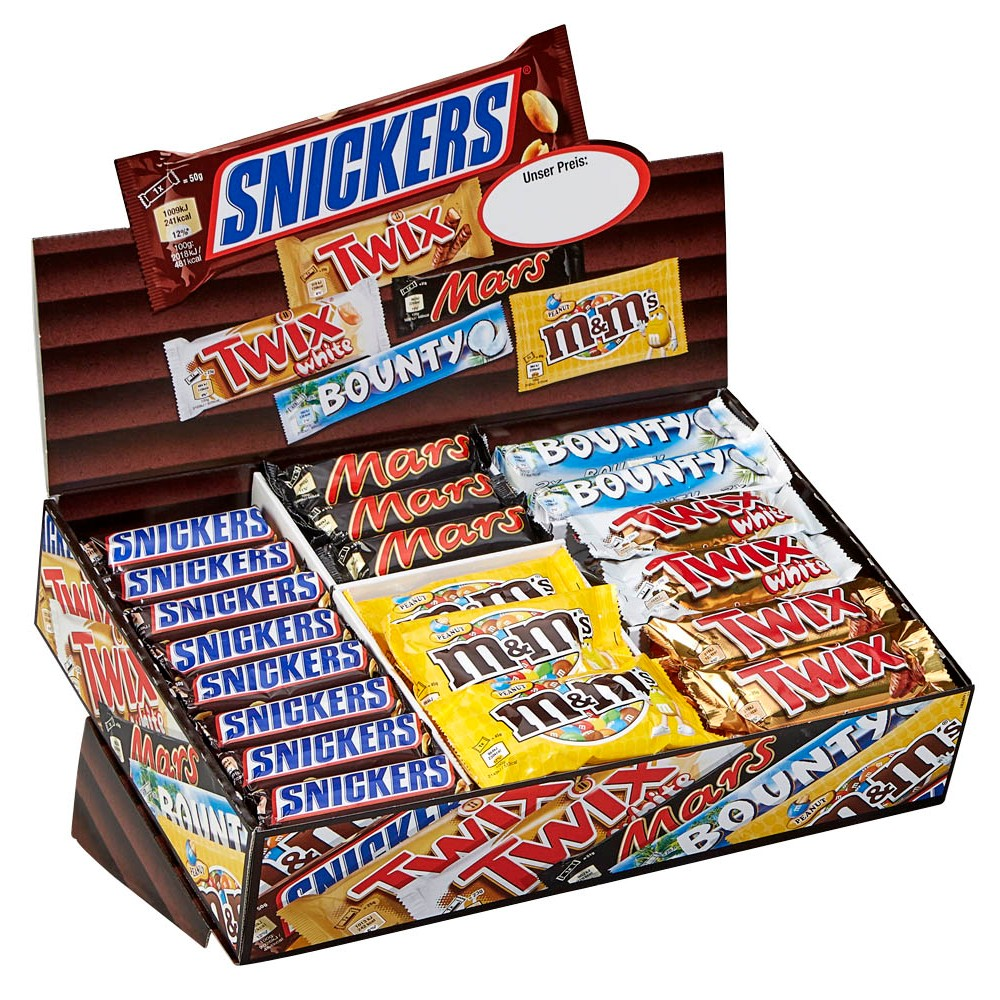
\includegraphics[width=0.3\textwidth, trim=0px 0px 0px -20px, clip] {fig/workObjects/all.jpeg}
   \label{fig:subfig1}
}
\subfigure[]{
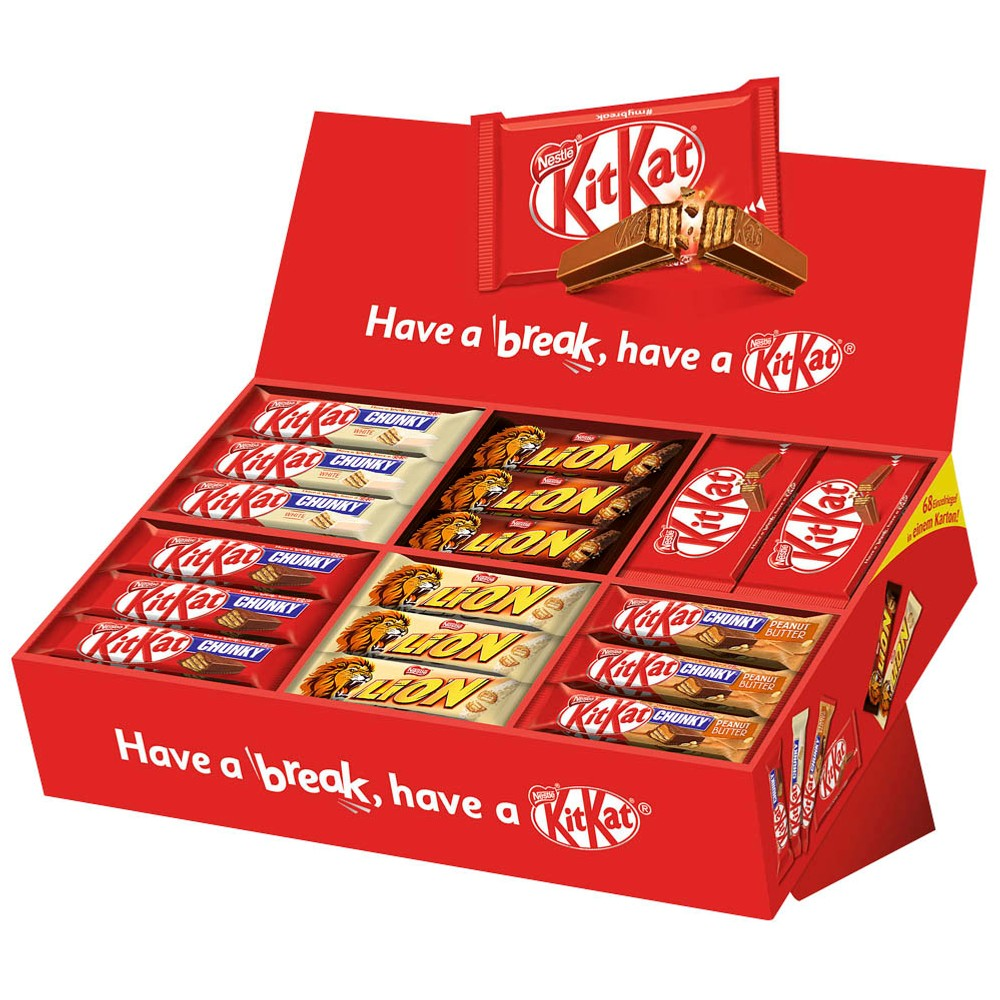
\includegraphics[width=0.3\textwidth, trim=0px 0px 0px -20px, clip] {fig/workObjects/nestle.jpeg}
   \label{fig:subfig2}
}
\subfigure[]{
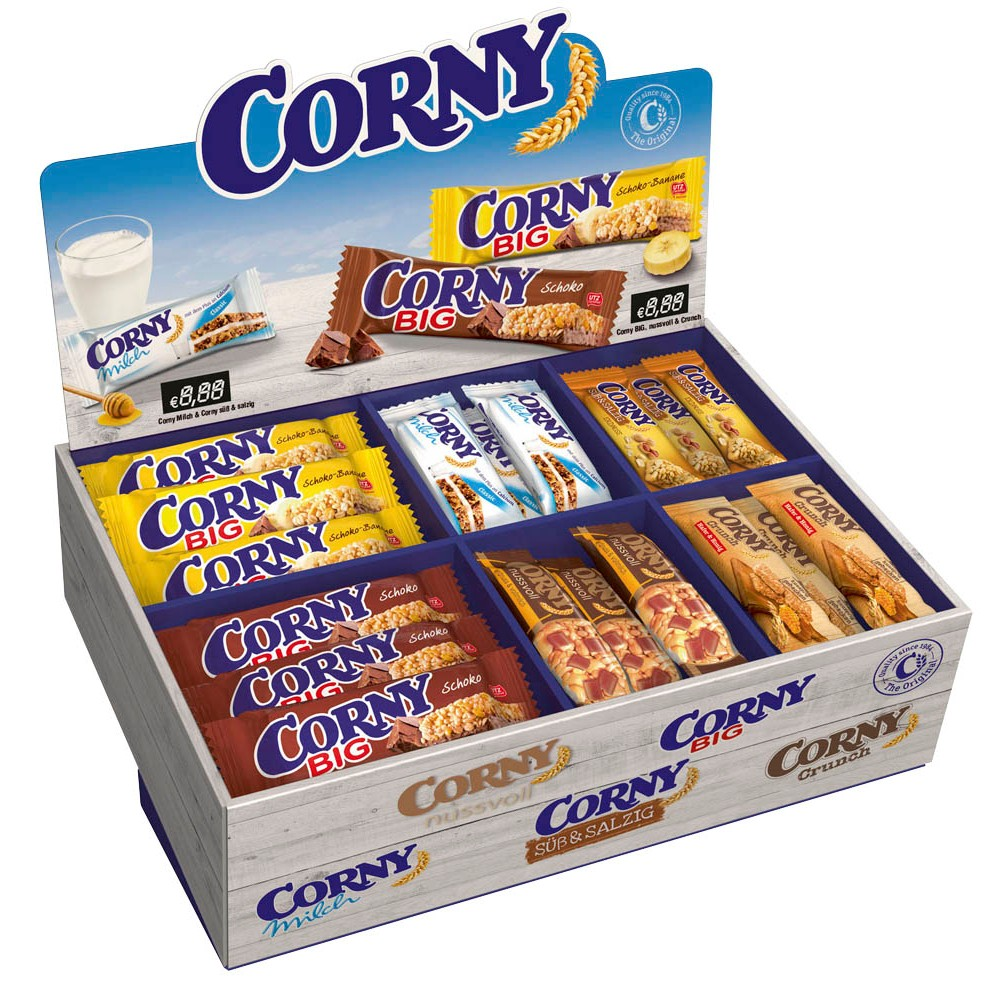
\includegraphics[width=0.3\textwidth, trim=0px 0px 0px -20px, clip] {fig/workObjects/corny.jpeg}
   \label{fig:subfig3}
}
\caption[Chocolate Objects (https://www.sweet24.de/)]{Chocolate objects }
\label{fig:labelHere}
\end{figure}
%--------------------------------------------------------------------
% EOF
%--------------------------------------------------------------------
